\section{A rank-one curve with unique arithmetic codes}\label{sec:elliptic}

This section supplies unique polynomial codes for the rational points of
a rank-one elliptic curve. Its group structure provides the integer index
used by the height construction in Section~\ref{sec:growth}. We first
record that structure, then implement rational coordinates and the group
law using the single-fold conventions of Section~\ref{sec:conventions}.

\subsection{The curve and its rational points}

Let
\[
 E:\quad y^2=x^3-25x
\]
denote the nonsingular projective cubic obtained by adjoining
\(O=[0:1:0]\) to this affine equation.  We use its chord--tangent group
law with identity \(O\).  Negation sends \((x,y)\) to \((x,-y)\).

\begin{proposition}\label{prop:rank-one}
The group \(E(\QQ)\) has rank one and torsion subgroup
\[
 \mathcal T=\{O,(0,0),(5,0),(-5,0)\}.
\]
Consequently there exists \(P\in E(\QQ)\) such that every rational
point has a unique expression \(nP+t\), with \(n\in\ZZ\) and
\(t\in\mathcal T\).
\end{proposition}

A complete two-isogeny descent proof is given in
Appendix~\ref{app:rank-one}. The construction below uses the group
decomposition in the proposition and the explicit torsion points.

\subsection{Unique codes for rational coordinates}

We must count all coordinates of a rational-point computation, including
the witnesses for reducedness.  Restricting a B\'ezout coefficient to one
residue interval is a standard way to make coprimality witnesses unique;
see \cite[Section~2]{cco2024}.  The following shifted inverse identity
also handles denominator one without a separate case.
A rational number is represented by six
natural numbers \((p,n,d,t,s,q)\) satisfying
\begin{equation}\label{eq:rational-code}
 pn=0,\qquad d=1+t+s,\qquad (p+n)t+d=1+qd.
\end{equation}
Its value is \((p-n)/d\).  The denominator is positive and
\(0\le t<d\); the last equation asserts that \(t\) is an
inverse of \(p+n\) modulo \(d\).

\begin{lemma}\label{lem:rational-codes}
Every rational number has exactly one code satisfying
\eqref{eq:rational-code}.  Any fixed finite sequence of rational
additions, subtractions, multiplications, divisions by nonzero divisors,
and comparisons on valid codes has a polynomial implementation with
unique outputs and auxiliary coordinates.
\end{lemma}

\begin{proof}
Put \(a=p+n\).  Equation~\eqref{eq:rational-code} gives
\(\gcd(a,d)=1\), so the represented fraction is reduced.
The constraint \(pn=0\) uniquely splits its numerator into its
positive and negative parts.  Conversely a reduced fraction with
positive denominator fixes \(p,n,d\).  If \(d>1\), its inverse
modulo \(d\) has exactly one representative \(t\) in
\([0,d-1]\); then
\[
 s=d-1-t,\qquad q=\frac{(p+n)t+d-1}{d}
\]
are uniquely determined nonnegative integers.  If \(d=1\), the
equations force \(t=s=q=0\).  In particular the unique code of
zero is \((0,0,1,0,0,0)\).

Clear positive denominators in any prescribed rational arithmetic
equation.  For instance, if the signed numerator and denominator of
the \(i\)-th code are \(a_i,d_i\), the equation
\(z_1+z_2=z_3\) becomes
\(a_1d_2d_3+a_2d_1d_3=a_3d_1d_2\).
The same procedure applies to products and to any fixed rational
expression whose denominators are known to be nonzero.  A comparison
becomes an integer polynomial comparison after multiplication by
positive denominators, and has a unique slack as in
Section~\ref{sec:conventions}.  When the resulting rational value
is uniquely specified, its entire code is unique by the first part.
\end{proof}

A point code consists of two valid rational codes and a flag
\(o\in\{0,1\}\).  For \(o=1\), force both rational numerators
to zero; this gives the unique dummy coordinate pair \((0,0)\)
and represents \(O\).  For \(o=0\), impose the affine curve
equation.  More explicitly, if the coordinate numerators and
denominators are \(a_x,d_x,a_y,d_y\), this equation is
\[
 a_y^2d_x^3=d_y^2(a_x^3-25a_xd_x^2).
\]
The implications are imposed by multiplication by \(o\) or
\(1-o\).  Thus every point of \(E(\QQ)\) has exactly one
point code; the flag distinguishes \(O\) from the affine point
\((0,0)\).

\begin{lemma}\label{lem:point-arithmetic}
Given valid codes for \(Q_1,Q_2\in E(\QQ)\), addition has a
polynomial implementation with a unique output code for \(Q_1+Q_2\)
and a unique complete tuple of auxiliary coordinates.  The same is
true of any fixed finite chain of additions and of multiplication by
any fixed positive integer.
\end{lemma}

\begin{proof}
The output is a shared valid point code.  Use the following disjoint
cases, with their guards included in the corresponding systems:
\begin{enumerate}
\item \(Q_1=O\): return \(Q_2\).
\item \(Q_1\ne O\), \(Q_2=O\): return \(Q_1\).
\item Both inputs affine and \(x_1<x_2\).
\item Both inputs affine and \(x_1>x_2\).
\item Both inputs affine, \(x_1=x_2\), and \(y_1+y_2=0\):
      return \(O\).
\item Both inputs affine, \(x_1=x_2\), \(y_1=y_2>0\).
\item Both inputs affine, \(x_1=x_2\), \(y_1=y_2<0\).
\end{enumerate}
At equal x-coordinates the curve equation gives
\(y_1^2=y_2^2\).  If the points are not negatives, they therefore
have equal nonzero y-coordinates.  This proves that the list is
exhaustive as well as disjoint.

In Cases 3 and 4 introduce a case-local rational slope code and impose
\[
 \lambda(x_2-x_1)=y_2-y_1.
\]
In Cases 6 and 7 instead impose
\[
 2y_1\lambda=3x_1^2-25.
\]
The coefficient of \(\lambda\) is nonzero in each case, so its
value and complete code are unique.  In all four cases require an
affine output and impose
\[
 x_3=\lambda^2-x_1-x_2,\qquad
 y_3=\lambda(x_1-x_3)-y_1.
\]
These are the chord--tangent formulas; they give the required point
on the curve.  Cases 1, 2, and 5 specify their output directly.

Apply the gated-case construction of Section~\ref{sec:conventions}.
In particular, the reducedness equations for a local slope code are
gated along with its other equations, and every coordinate of an
inactive slope code is forced to zero.  Only the shared output code
remains globally valid.  Thus no inactive branch contributes a
choice.  Lemma~\ref{lem:rational-codes} gives uniqueness of every
active arithmetic witness.  Induction along a fixed finite chain
proves the final assertions.
\end{proof}

Fixed rational points may now be inserted by their fixed integer
codes.  We henceforth fix \(P\) as in
Proposition~\ref{prop:rank-one}, as well as the four points of
\(\mathcal T\).  No assertion that the construction numerically
computes this choice of \(P\) is needed.

\section{A uniquely represented function with intermediate growth}
\label{sec:growth}

We now use the curve to construct a total single-fold function whose
growth is faster than every fixed power and slower than \(u^u\).
The group decomposition provides an integer index, but the polynomial
systems will quantify only uniquely coded rational points.  A height
comparison will select both a point at a given scale and a second
point whose index is the square of the first.
Rank-one elliptic curves have been used in Diophantine definability;
see Poonen \cite{poonen2002}.  Here we use the full rational
x-height: its bounded logarithmic error permits an exact comparison of
integer indices.  The construction below proves the required
single-fold graph directly.

\subsection{Uniform heights and representatives}

For a reduced rational number \(a/d\) with \(d>0\), define
\[
 H(a/d)=\max\{|a|,d\}.
\]
Put \(h_x(Q)=\log H(x(Q))\) for affine \(Q\), and
\(h_x(O)=0\).  We use the canonical height with normalization
\[
 \widehat h(Q)=\frac12\lim_{N\to\infty}
                  4^{-N}h_x([2^N]Q).
\]
The N\'eron--Tate canonical-height theorem gives existence of this limit,
\(\widehat h([j]Q)=j^2\widehat h(Q)\), and
\(\widehat h(Q)>0\) for nontorsion rational \(Q\).
Since \(x\) is an even function of degree two, it also gives a
constant \(c_E>0\), depending only on this curve and coordinate,
such that
\begin{equation}\label{eq:uniform-height}
 \bigl|\log H(x(Q))-2\widehat h(Q)\bigr|\le c_E
 \qquad(Q\in E(\QQ),\ Q\ne O).
\end{equation}
These are precisely the uniform comparison and quadraticity statements
of \cite[Chapter~VIII, Proposition~9.1 and Theorem~9.3]{silverman}.

We will compare a bounded height error with the gap between distinct
integer indices. A fixed scalar multiplication enlarges the quadratic
coefficient while leaving the uniform error bound unchanged. Choose an
integer \(\kappa>e^{6c_E}\), then choose a positive even integer \(m_*\)
so large that \(a_E=2m_*^2\widehat h(P)\) satisfies
\begin{equation}\label{eq:height-constants}
 a_E>2c_E,
 \qquad 2a_E-6c_E>\log\kappa.
\end{equation}
Such a choice exists because \(\widehat h(P)>0\).

Define a positive integer-valued function on rational points by
\[
 W(Q)=
 \begin{cases}
 H(x([m_*]Q)),&[m_*]Q\ne O,\\
 1,&[m_*]Q=O.
 \end{cases}
\]
It has a unique polynomial computation from the point code: compute
\([m_*]Q\) using Lemma~\ref{lem:point-arithmetic}, and take the
maximum of the absolute numerator \(p+n\) and denominator \(d\)
in its x-code.  The dummy x-code at infinity gives the same value
one.  The two disjoint comparisons used to compute a maximum have
unique slacks and selectors.

Because \(m_*\) kills \(\mathcal T\), the value of
\(W(nP+t)\) depends only on \(j=|n|\).  Denote it by \(W_j\).
Then
\begin{equation}\label{eq:quadratic-sequence}
 W_0=1,\qquad
 \log W_j=a_Ej^2+\varepsilon_j,
 \quad |\varepsilon_j|\le c_E\quad(j\ge1).
\end{equation}
In particular \(W_1>1\).  For \(j\ge1\) the successive
logarithmic difference is at least
\(a_E(2j+1)-2c_E>0\).  Hence \((W_j)_{j\ge0}\) is strictly
increasing and unbounded.

We next choose one point for each positive absolute index.  Call a
rational point \(Q\) a \emph{representative} if it satisfies
\begin{equation}\label{eq:representative}
 \begin{gathered}
 Q\ne O,\qquad y(Q)\ge0,\qquad W(Q)>1,\\
 Q+t\ne O\quad\hbox{and}\quad x(Q)\ge x(Q+t)
       \qquad(t\in\mathcal T).
 \end{gathered}
\end{equation}
This is a finite polynomial system on its point code, with unique
auxiliaries for each point satisfying it: there are only four
translates, and their addition and comparison computations are unique.

\begin{lemma}\label{lem:representatives}
For each integer \(j\ge1\), exactly one point in
\((jP+\mathcal T)\cup(-jP+\mathcal T)\) satisfies
\eqref{eq:representative}.  These are all the representatives.
\end{lemma}

\begin{proof}
The condition \(W(Q)>1\) excludes exactly the torsion points by
\eqref{eq:quadratic-sequence}.  Every translate of a nontorsion
point by torsion is affine.  In a coset \(jP+\mathcal T\),
\(j\ne0\), the x-coordinates are distinct: equality of two
x-coordinates on the short Weierstrass curve means that the points
are equal or negatives.  Equality identifies the torsion translates;
the negative possibility would imply that \(2jP\) is torsion.

The finite coset therefore has a unique point of maximal x-coordinate.
The inequalities in \eqref{eq:representative} pick precisely this
point.  Negation sends it to the unique maximal point in the opposite
coset, since negation preserves x and permutes \(\mathcal T\).
Neither maximal point has y-coordinate zero, because such points
are torsion.  Exactly one of the two has positive y-coordinate.
This proves the claim, including exhaustiveness by
Proposition~\ref{prop:rank-one}.
\end{proof}

\subsection{Selecting and squaring an index}

The next construction specifies its points by finitely many height
comparisons.  Its proof of uniqueness uses the index in
\(E(\QQ)/\mathcal T\); that index is not an additional
variable of the polynomial system.

\begin{proposition}\label{prop:growth}
There are a total function \(g:\NN\to\NN\), a real constant
\(\delta>0\), and an integer \(u_0\ge4\) such that the graph
of \(g\) has a single-fold Diophantine representation, including
uniqueness of its output and every auxiliary coordinate for each
input, and
\begin{equation}\label{eq:growth-bounds}
 \delta(\log u)^2<\log g(u)<u\log u
       \qquad(u\ge u_0).
\end{equation}
\end{proposition}

\begin{proof}
\emph{Selecting an index at the input scale.}
The integer \(W_1=W(P)\) is now fixed.  On input \(u\in\NN\),
require a representative \(Q\) satisfying
\begin{equation}\label{eq:index-bracket}
 W(Q)\le u+W_1<
          \max\{W(Q+P),W(Q-P)\}.
\end{equation}
If \(Q\) has absolute index \(k\ge1\), its two neighbors
have W-values \(W_{k-1}\) and \(W_{k+1}\), in some order.
Thus their maximum is \(W_{k+1}\).  Since the sequence is
strictly increasing and unbounded, and \(u+W_1\ge W_1\),
there is exactly one \(k\ge1\) such that
\[
 W_k\le u+W_1<W_{k+1}.
\]
Lemma~\ref{lem:representatives} then gives exactly one permissible
point \(Q\).  This reasoning includes \(u=0\), for which
\(k=1\).

\smallskip
\noindent\emph{Selecting the squared index.}
Require a second representative \(R\). To derive the comparisons that
will determine it, write \(r\ge1\) for its absolute index. Like \(k\),
this is notation for the proof, not a variable of the system. We want
to impose \(r=k^2\) using only point operations and height comparisons.
The quadratic main terms in \eqref{eq:quadratic-sequence} suggest the
identity
\[
 (2k)^2-2k^2-\bigl((r+1)^2-r^2\bigr)+1=2(k^2-r).
\]
Thus the first difference in \(r\) cancels its quadratic term, while
doubling \(k\) leaves a multiple of \(k^2\). The same linear combination
of logarithmic heights therefore tests \(k^2-r=0\) with bounded error.
Products express this test without logarithms: using the
unique point and height computations, form the positive integers
\begin{align*}
 L_0&=W([2]Q)\,W(R)\,W_1,\\
 D_0&=W(Q)^2\max\{W(R+P),W(R-P)\},
\end{align*}
and impose
\begin{equation}\label{eq:square-window}
 L_0\le\kappa D_0,\qquad D_0\le\kappa L_0.
\end{equation}
The neighbor maximum in \(D_0\) equals \(W_{r+1}\), by the same
argument as for \(Q\). All indices in the following calculation are
positive, so
\eqref{eq:quadratic-sequence} gives
\begin{align*}
 \log\frac{L_0}{D_0}
 &=a_E\bigl((2k)^2+r^2+1-2k^2-(r+1)^2\bigr)+e\\
 &=2a_E(k^2-r)+e,\qquad |e|\le6c_E.
\end{align*}
The error has six terms when multiplicity is counted: one each from
\(W_{2k},W_r,W_1,W_{r+1}\), and two from \(W_k\).
If \(r=k^2\), its absolute value is less than \(\log\kappa\),
so \eqref{eq:square-window} holds.  If \(r\ne k^2\), integer
separation and \eqref{eq:height-constants} give
\[
 \left|\log\frac{L_0}{D_0}\right|
     \ge2a_E-6c_E>\log\kappa,
\]
so the window fails.  Therefore exactly the representative of
absolute index \(k^2\) can serve as \(R\).
Figure~\ref{fig:height-window} illustrates this separation.

\smallskip
\noindent\emph{Totality and unique witnesses.}
Set the output to
\[
 g(u)=W(R)=W_{k^2}.
\]
The construction uses only fixed addition chains, rational point
codes, maxima, products, and comparisons.  It is therefore a finite
polynomial system.  For every \(u\), the bracket pins \(Q\)
and the window pins \(R\).  Once these points are fixed, their
complete codes, every intermediate point and height, all comparison
slacks, and all branch selectors are fixed.  Lemmas
\ref{lem:rational-codes} and \ref{lem:point-arithmetic}, together
with the inactive-variable convention, give uniqueness of every
expanded auxiliary.  Conversely those uniquely specified points and
computations satisfy the system.  This proves totality and the
single-fold assertion before any asymptotic cutoff is chosen.

\smallskip
\noindent\emph{Growth estimates.}
Write \(U=u+W_1\). The
bracket and \eqref{eq:quadratic-sequence} imply
\begin{equation}\label{eq:index-growth-estimate}
 a_Ek^2-c_E\le\log U
   <a_E(k+1)^2+c_E\le4a_Ek^2+c_E.
\end{equation}
For all sufficiently large \(u\), the upper estimate on \(\log U\)
gives \(k^2>\log u/(8a_E)\).  Hence
\[
 \log g(u)\ge a_Ek^4-c_E
       >\frac{(\log u)^2}{128a_E}
\]
eventually.  We may take \(\delta=1/(128a_E)\).
The other estimate in \eqref{eq:index-growth-estimate} gives
\[
 \log g(u)\le a_Ek^4+c_E
    \le\frac{(\log(u+W_1)+c_E)^2}{a_E}+c_E
    =O((\log u)^2).
\]
This is eventually strictly less than \(u\log u\).
Choose an integer \(u_0\ge4\) beyond both thresholds, proving
\eqref{eq:growth-bounds}.
\end{proof}

The real constants used in the estimates are not variables or
coefficients of the polynomial system.  They justify choices of
fixed integers, while all fixed rational points enter through integer
codes.  Proposition~\ref{prop:growth} is thus an existence statement
about an integer polynomial; no numerical determination of a generator
or of the height constants is asserted.

\begin{figure}[tbp]
\centering
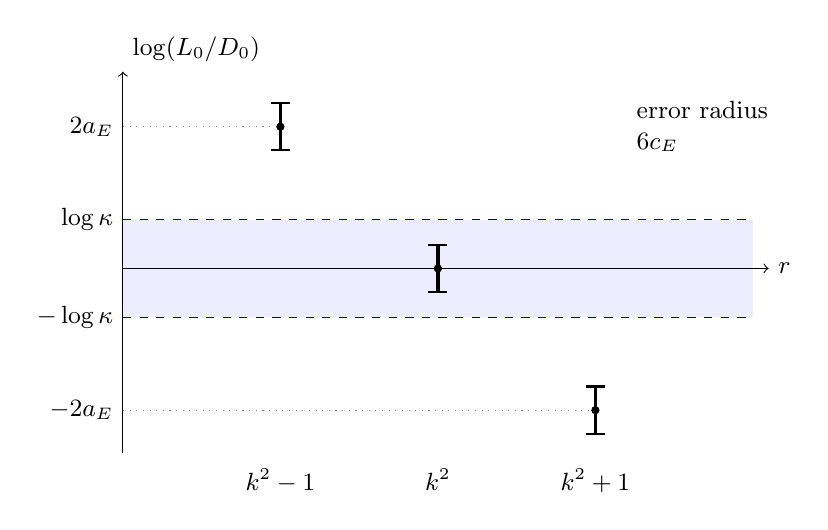
\begin{tikzpicture}[x=1cm,y=1cm,font=\small]
  \fill[blue!7] (1,-.62) rectangle (9,.62);
  \draw[blue!55!black,dashed] (1,.62)--(9,.62);
  \draw[blue!55!black,dashed] (1,-.62)--(9,-.62);
  \draw[->] (1,-2.35)--(1,2.5)
    node[above right] {$\log(L_0/D_0)$};
  \draw[->] (1,0)--(9.2,0) node[right] {$r$};
  \node[left] at (1,.62) {$\log\kappa$};
  \node[left] at (1,-.62) {$-\log\kappa$};
  \draw[gray,dotted] (1,1.8)--(3,1.8);
  \draw[gray,dotted] (1,-1.8)--(7,-1.8);
  \node[left] at (1,1.8) {$2a_E$};
  \node[left] at (1,-1.8) {$-2a_E$};
  \foreach \x/\y in {3/1.8,5/0,7/-1.8}{
    \draw[very thick] (\x,\y-.30)--(\x,\y+.30);
    \draw[thick] (\x-.12,\y-.30)--(\x+.12,\y-.30);
    \draw[thick] (\x-.12,\y+.30)--(\x+.12,\y+.30);
    \fill (\x,\y) circle (1.5pt);
  }
  \node[below] at (3,-2.42) {$k^2-1$};
  \node[below] at (5,-2.42) {$k^2$};
  \node[below] at (7,-2.42) {$k^2+1$};
  \node[right,align=left] at (7.4,1.8) {error radius\\$6c_E$};
\end{tikzpicture}
\caption{The index window, schematically for \(k\ge2\). At index \(r\),
the logarithmic ratio lies within \(6c_E\) of \(2a_E(k^2-r)\).
The choice \(6c_E<\log\kappa<2a_E-6c_E\) puts the entire middle
interval in the admissible band and every other integer-index interval
outside it. The error bars represent bounds, not additional variables.}
\label{fig:height-window}
\end{figure}


The uniqueness assertion includes every intermediate point in every
fixed scalar chain, all six coordinates of each rational code, and every
nested comparison or branch witness. Inactive local tuples are zero.
Appendix~\ref{app:witnesses} specifies the complete tuple and follows it
through the power and computation constructions.
